\chapter{Tutorials}

\begin{figure}
	\centering
	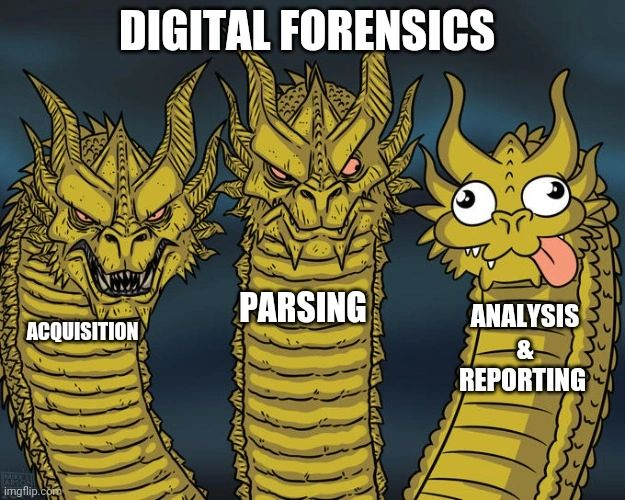
\includegraphics[scale=0.35]{appendix/images/digitalForensics.jpg}
	\caption{Test caption number}
\end{figure}

\section{LaTeX TUTORIALS}
\subsubsection{Citation \& Reference}
tutorial for referencing: This is a sample text \cite{daghmehchi2022memory} 

Exercises show two there are two parts to a citation: the citation; and the reference. There are many styles and configurations of the citations and references, which the exercises will make clear. 

Essentially, to start with, we are going to keep this simple and use the plain bibliography setting. As we advance the national bibliography package can be used and this is in the exercises on citations. This setting orders all bibliography items in alphabetical order and only uses the cite command. It does have its restrictions and we will come across these and how to cope with them. The following is an example paragraph using citations and a plain bibliography and should be adequate to get us started.


The first generation of Neural Networks are generally considered as Perceptrons \cite{rosenblatt1958perceptron}. Minsky and Papert \cite{minsky1969perceptrons} wrote a critique of the perceptron which showed that it could not solve non-linear problems, typically XOR. To solve the non-linear problem Rumelhart, Hinton and Williams \cite{rumelhart1985learning} made an enormous contribution with the Back-propagation error Artificial Neural Network, ANN. This and related ANN are generally referred to as second generation and inspire many of the techniques used in machine learning. The third generation of neural networks are based on biologically-inspired neurons and are generally referred to as, ``spiking neurons''.  Oddly many third generations are based on research pre-dating to first and second generations, namely Hebbian Learning \cite{Hebb}. These spiking neurons can be built into bigger networks to solve complex problems, e.g., see \cite{huyck2013compensatory}.

\subsubsection{Example of glossary}
There are several blockchain \gls{ca1} but three of interest are: \gls{poet}, \gls{pow} and \gls{pos}.

\gls{poet} is fast and can only be used on permission blockchains. \gls{pow} is computationally expensive and can be used on permissionless blockchains, many researchers have commented that \gls{pow} is unsustainable. \gls{pos} is less computationally expensive and can be used on permissionless blockchain technology. 

\subsubsection{Schedule}
You can reference the image as follows: Fig.\ref{fi:LinuxDir}.

% % % % % % % % % % % % % % %
%
%	INCLUDING FILES	
%	File: appendix/images/linux-directory-structure.png
%	N.B. 	This is compiled from the parent directory.
%		Hence referencing appendix/images directory from within appendix/images
% 
% % % % % % % % % % % % % % %
\begin{figure}
\centering
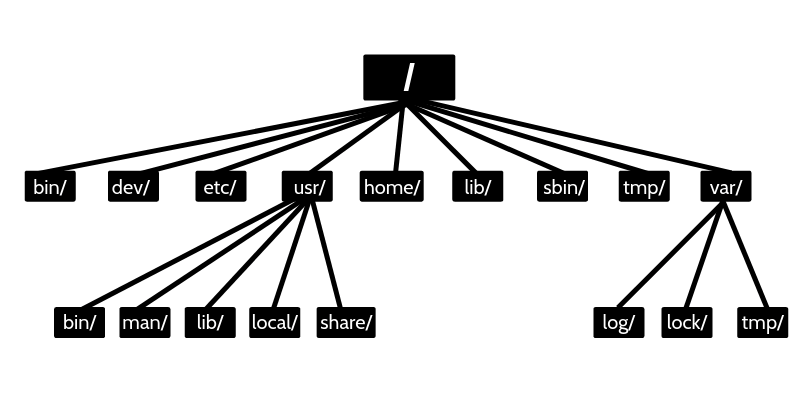
\includegraphics[scale=0.4]{appendix/images/linux-directory-structure.png}
\caption{Linux Directory Structure}\label{fi:LinuxDir}
\end{figure}


\begin{figure}
	\centering
	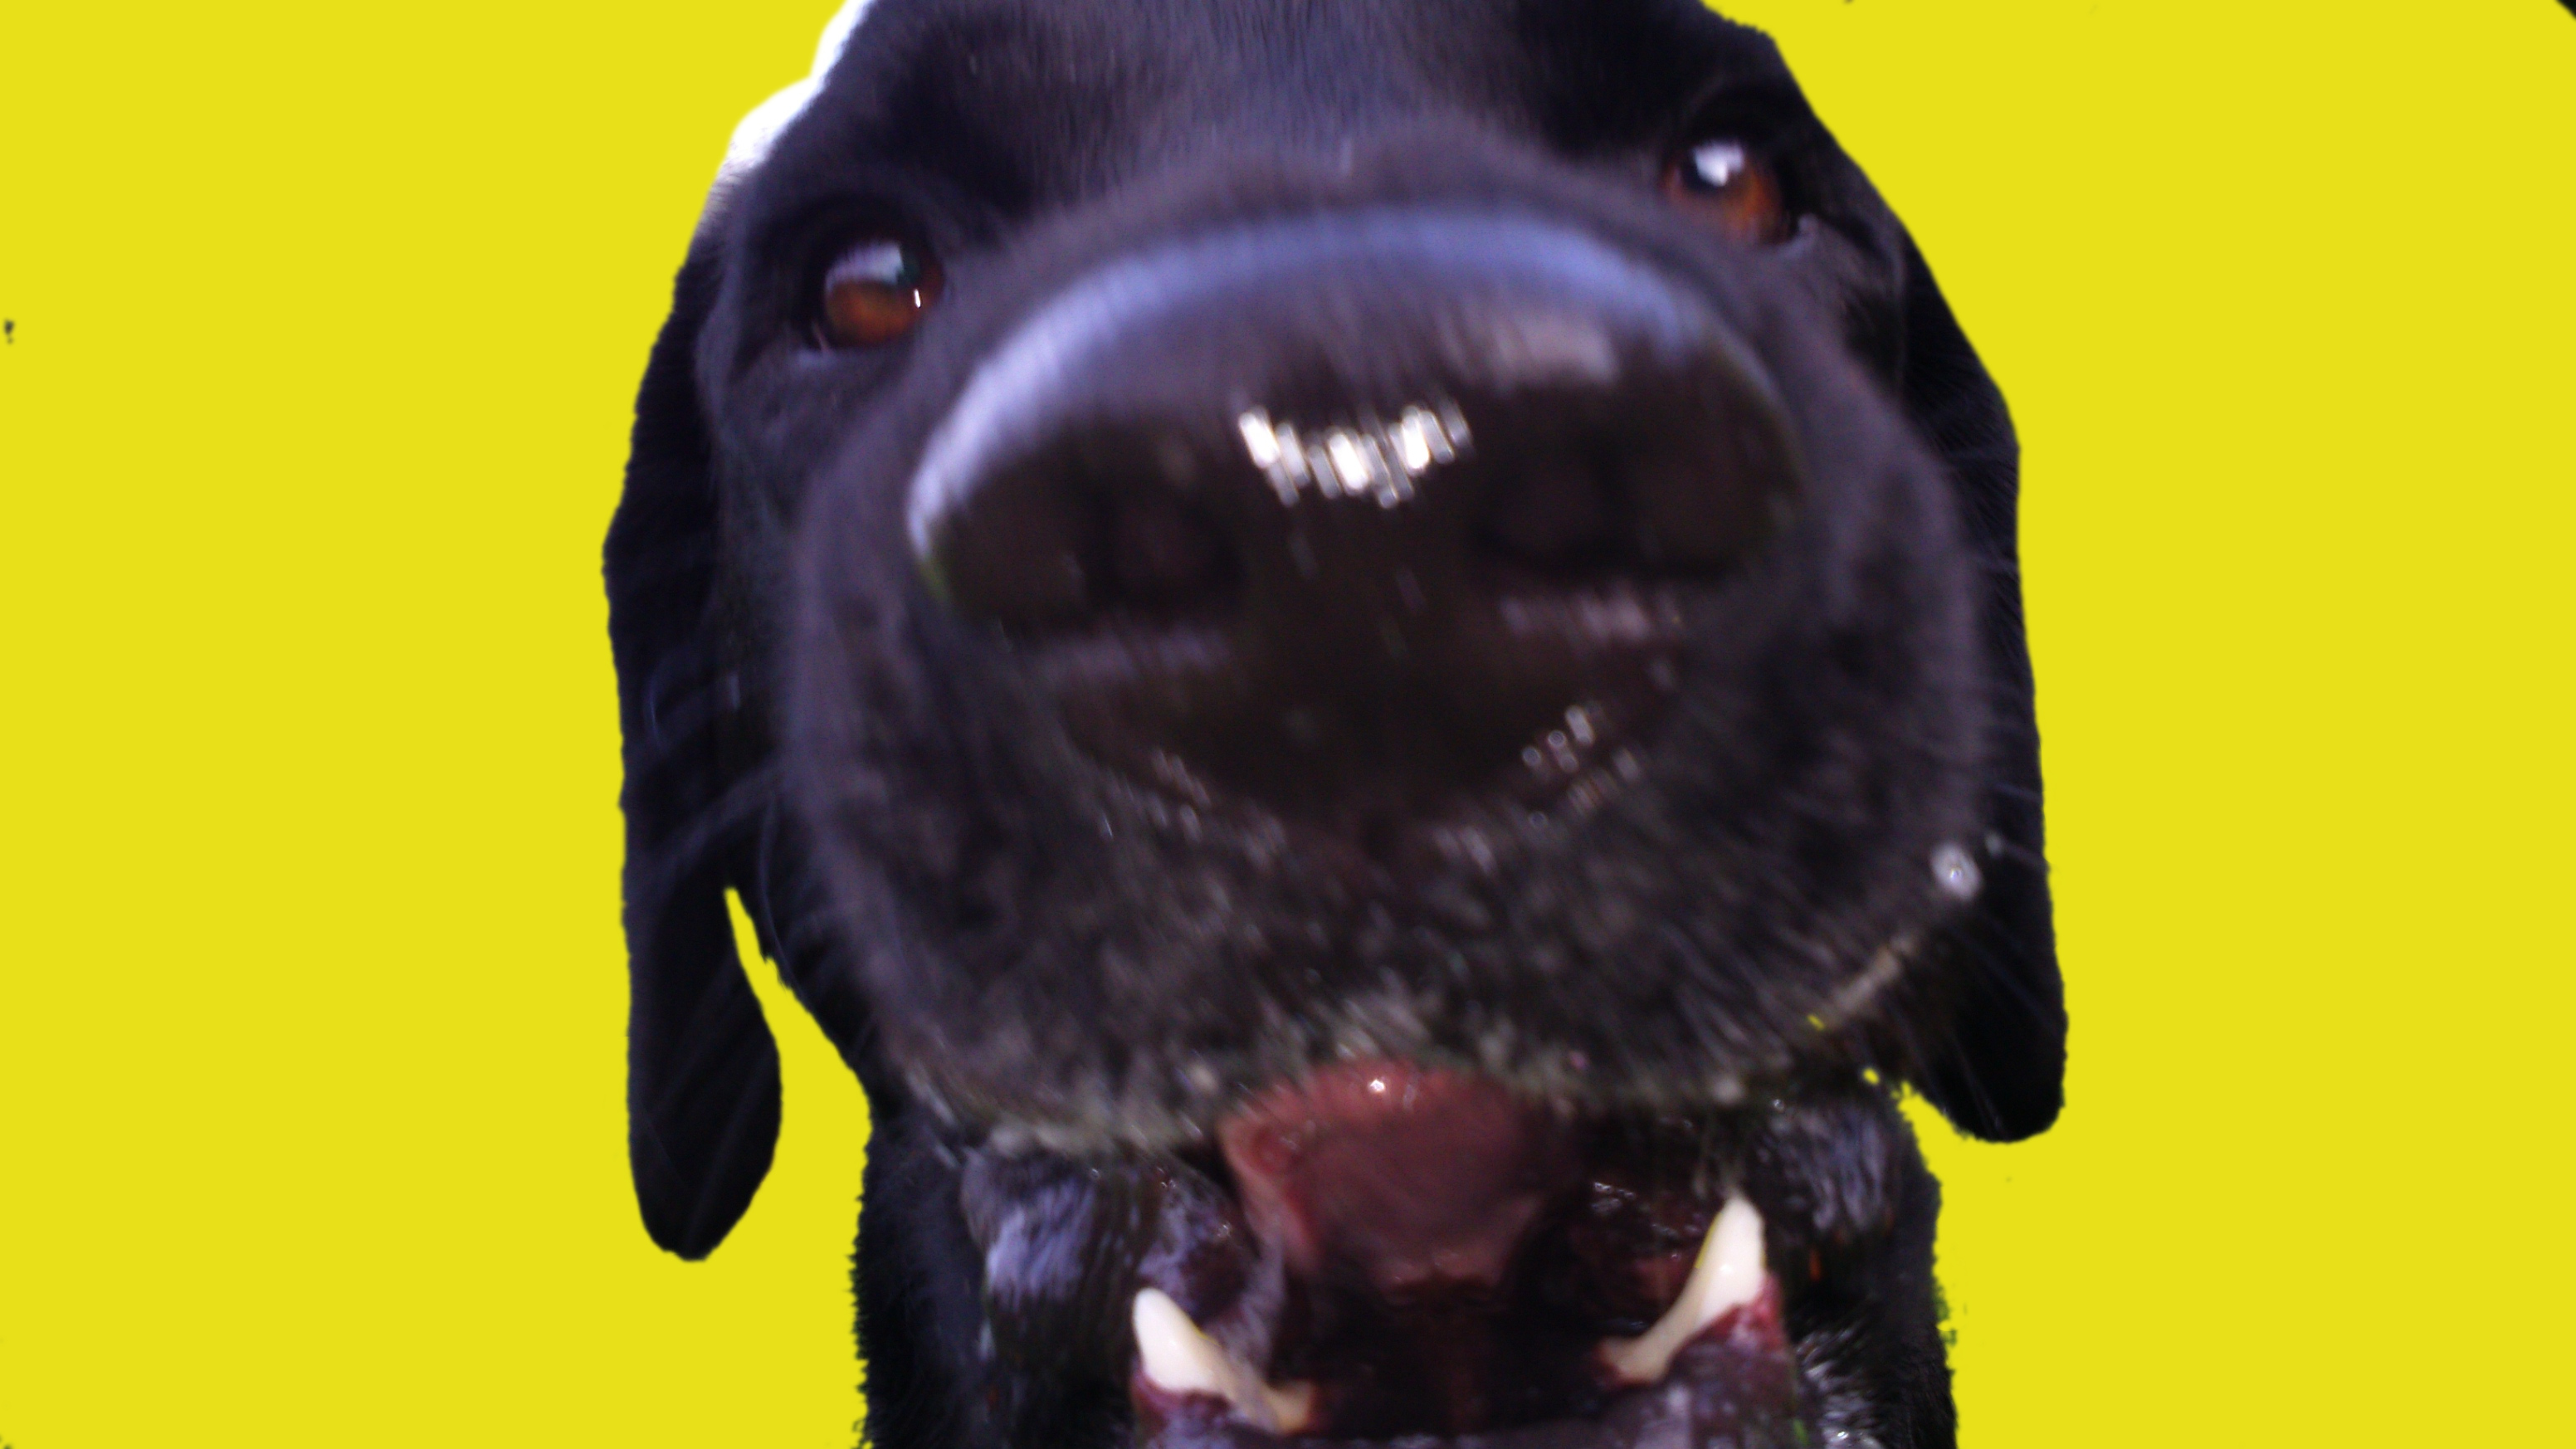
\includegraphics[scale=0.1]{appendix/images/awo}
	\caption{Test caption number}
\end{figure}

\newpage

\subsubsection{Experiment 1}
Use graphics to display results. Most results can be shown in tables. Use package longtables if you have trouble getting all data into a single page. Remember to label and reference the table.

\begin{table}
	\centering
	\begin{tabular}{|c|l|l|l||r|}\hline
	Run	&	x	&	y 	&	z	& Time/ms\\ \hline
	1	&	100	&	2.5	& 	1.06	& 60000 \\ \hline
	2	&	200	&	4.5	&	1.45	& 50000 \\ \hline
	3	&	500	&	5.5	&	1.5	& 40000 \\ \hline
	\end{tabular}
	\caption{Experiment 1 Results}
	\label{ta:ex1}
\end{table}


\subsubsection{Experiment 2}
Experiment 2 should differ from Experiment 1. Each experiment should be repeated a number of times for reproducibility. Do not confuse Experiment 2 as a repeat of Experiment 1, they are different. 

\begin{table}
	\centering
	\begin{tabular}{|c|l|l|l||r|}\hline
	Run	&	x	&	y 	&	z	& Time/ms\\ \hline
	1	&	100	&	2.5	& 	1.06	& 60000 \\ \hline
	2	&	200	&	4.5	&	1.45	& 50000 \\ \hline
	3	&	500	&	5.5	&	1.5	& 40000 \\ \hline
	\end{tabular}
	\caption{Experiment 2 Results}
	\label{ta:ex2}
\end{table}


\chapter{Ethical Approval}
The below form needs to be filled first, then signed by your supervisor.
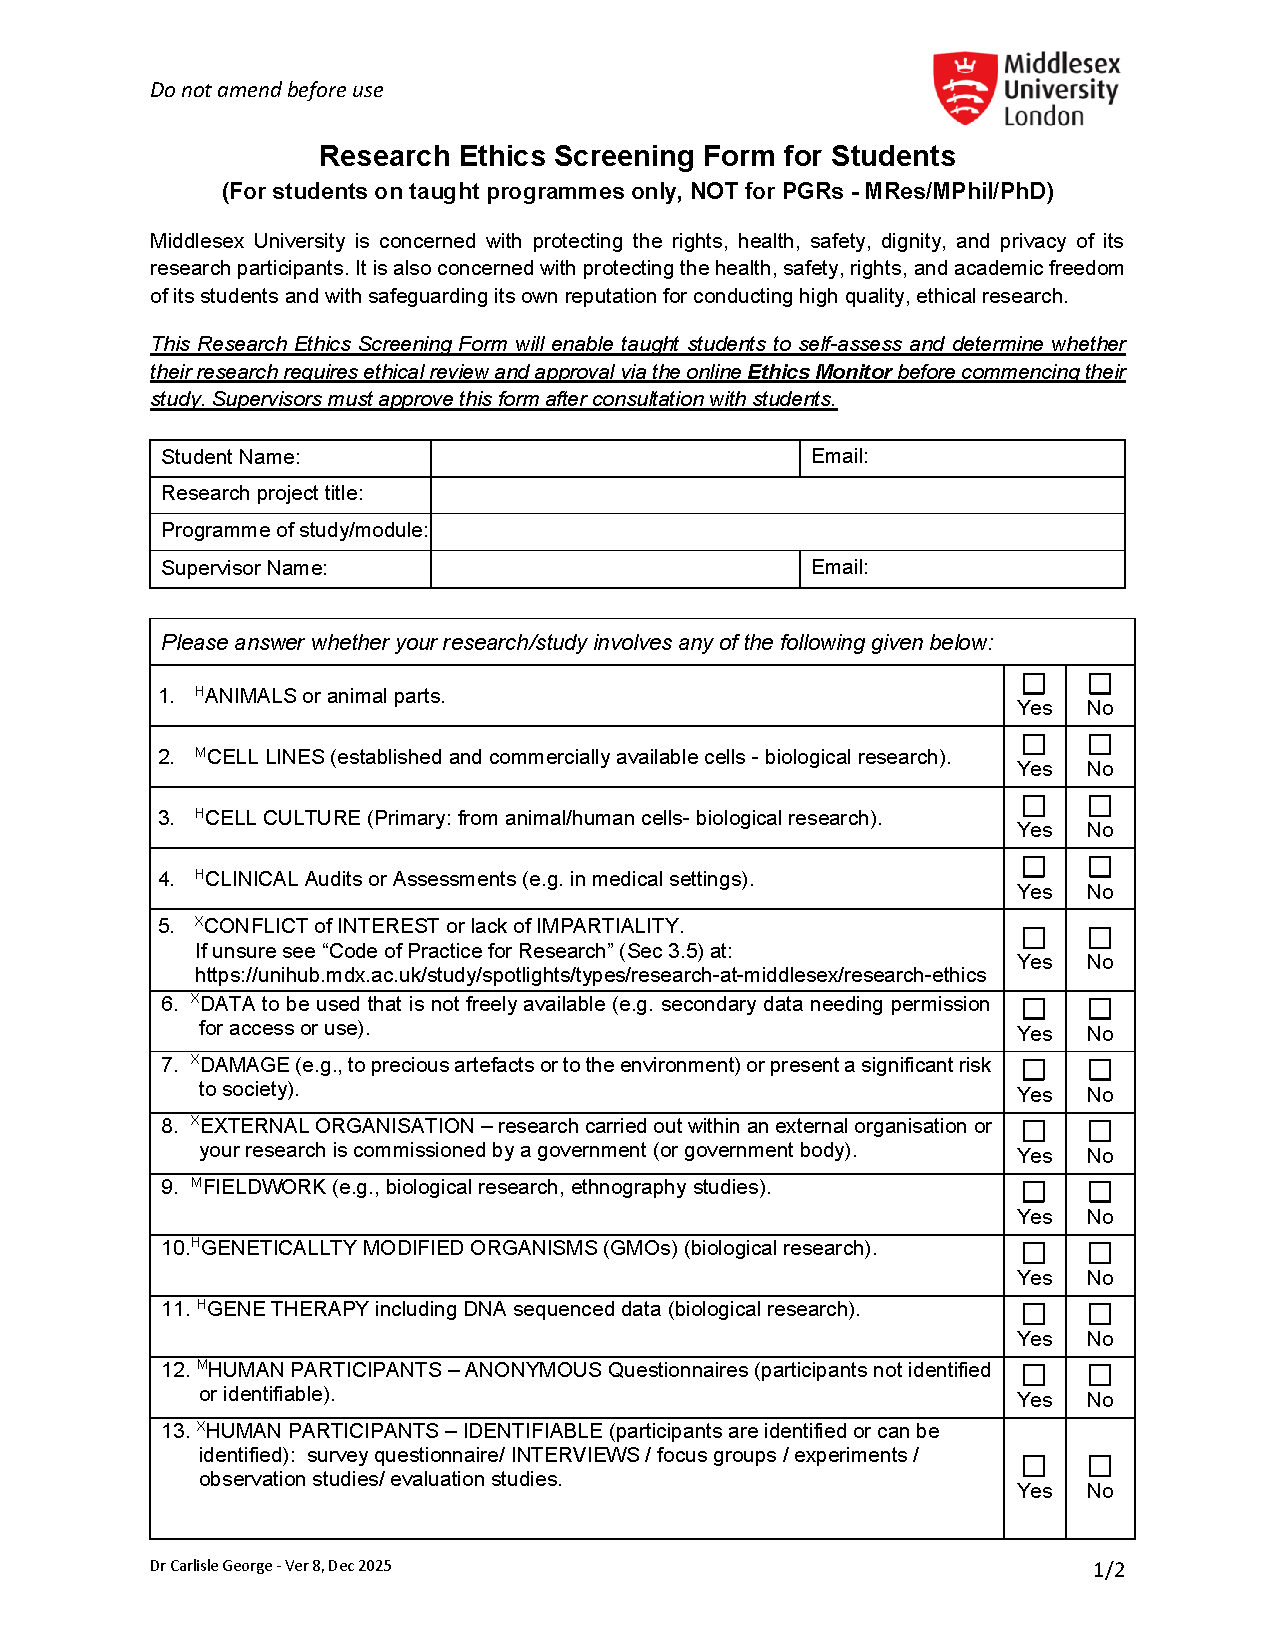
\includepdf[pages=-, scale=0.75]{appendix/MUR Research Ethics Screening Form for Students V8.pdf}

\chapter{Meeting Log with Supervisor}
%include pdf file, "meetings.pdf". 
% The options include only page 1, because it is already a4, it is scale down to 0.75. 
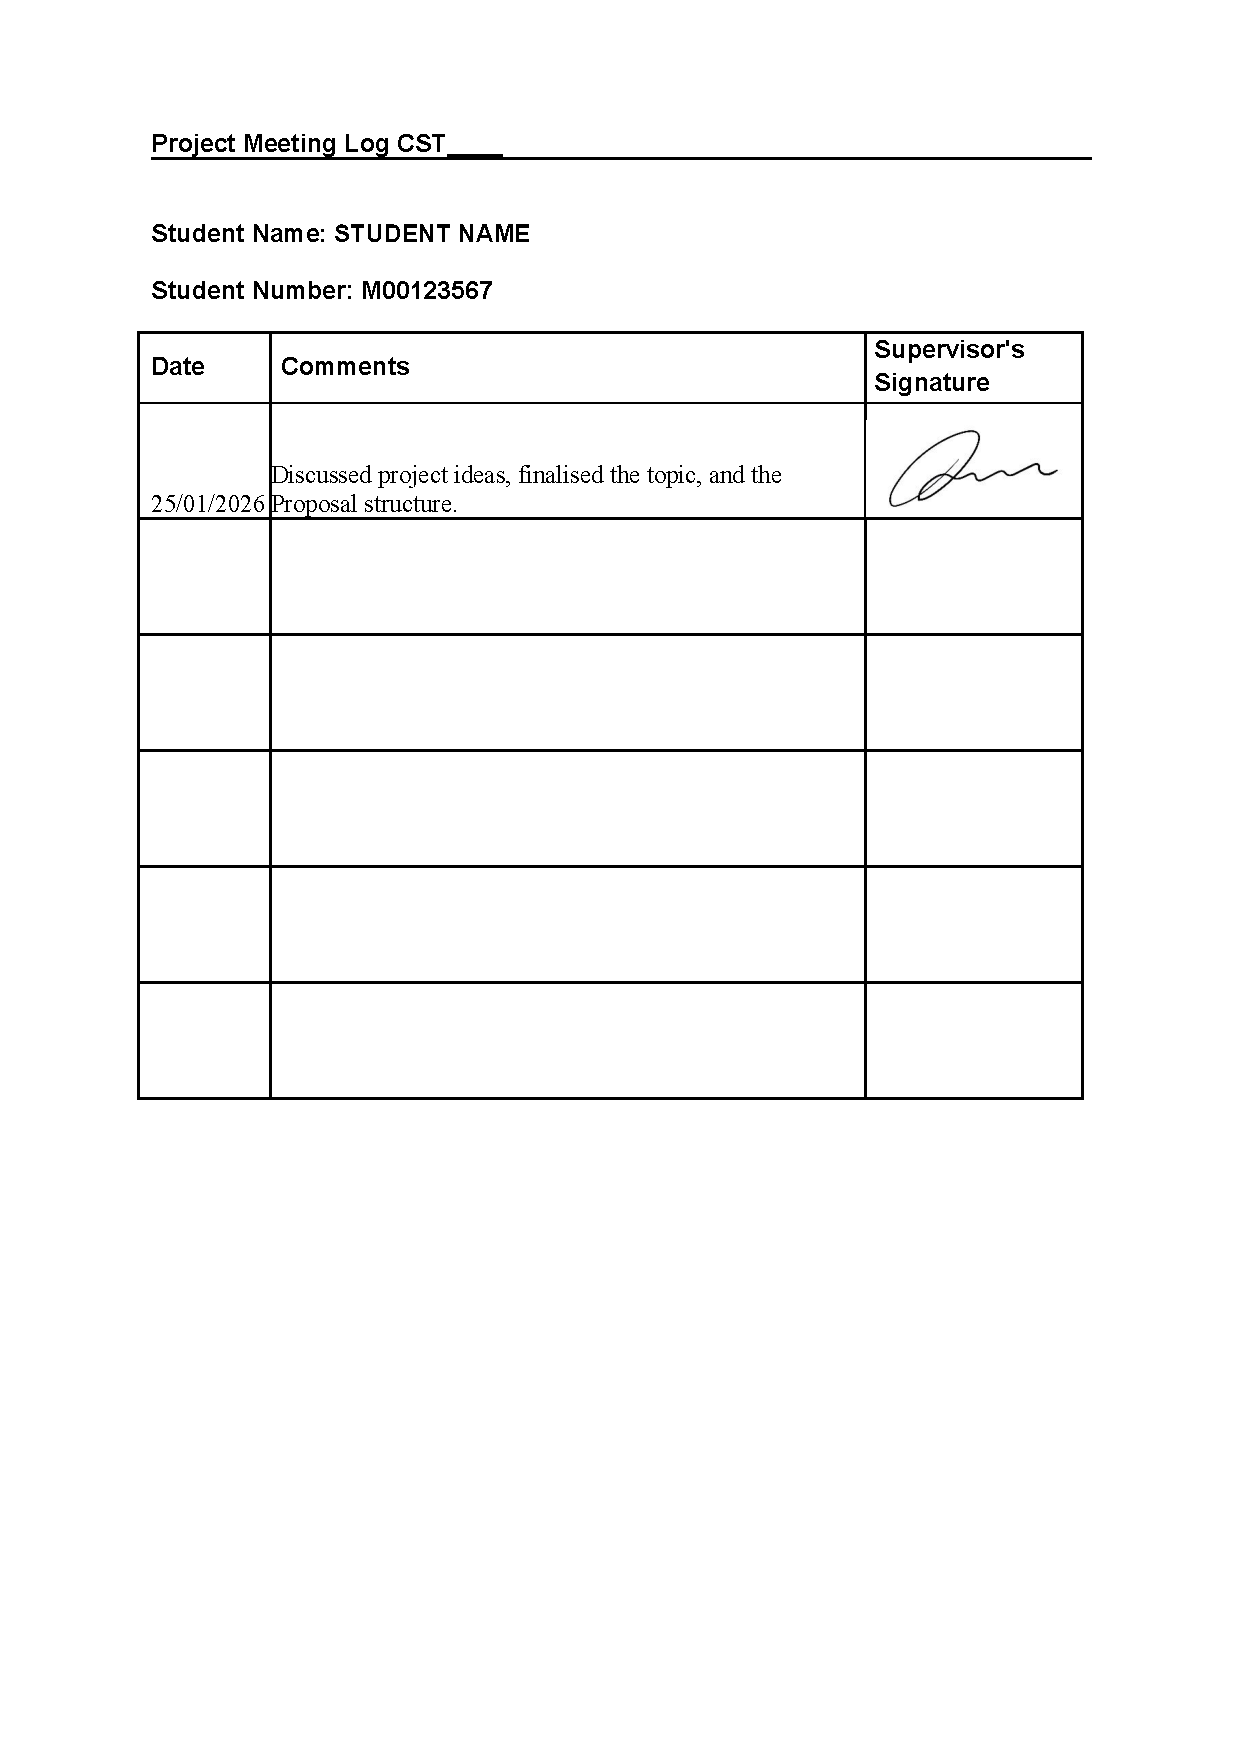
\includepdf[pages=1,scale=0.75]{appendix/Meeting Logs.pdf}